\documentclass{article}
\usepackage{amsmath, amsfonts, amsthm, amssymb}  
\usepackage{secdot}
\usepackage{epsfig}
\usepackage{cprotect}
\usepackage[T1]{fontenc}
\usepackage{epstopdf}
\usepackage{url}
\usepackage{rotating}
\usepackage{graphicx}
\usepackage{caption}
\usepackage{subcaption}
\usepackage{multirow}
\usepackage{setspace}
\usepackage{array}
\usepackage{fancyhdr}
\usepackage{lastpage}
\usepackage[T1]{fontenc}

\usepackage{geometry}
\geometry{letterpaper, left=1in, right=1in, top=1in, bottom=1in}

\pagestyle{fancy}
\fancyhf{}
\rhead{\thepage/\pageref{LastPage}}
\lhead{OSU ECEN 3233 - Logic Design - Spring 2022}
\rfoot{\LaTeX}


% ----- Identifying Information -----------------------------------------------
\newcommand{\myassignment}{Project: Crypto Cracking with Hardware}
\newcommand{\myduedate}{Assigned: Tuesday 3/28; Due \textbf{Saturday 4/30} (midnight)}
\newcommand{\myinstructor}{Instructor: James E. Stine, Jr.}
% -----------------------------------------------------------------------------

\begin{document}
\begin{center}
  {\huge \myassignment} \\
  {\large \myduedate} \\
  \begin{flushright}
  \myinstructor \\
  \end{flushright}
\end{center}

\section{Introduction}

This project is meant to be an encompassing project that gives you the
full experience of all that you learned in this course.  It will bring
ideas that we covered as well as had within laboratories.  It will
also try to reinforce all the skills you learned during your time in
laboratory.

We will revisit using security hardware again but in this setting we
will have an idea of what security system is in place.  For this
laboratory, you will revisit Laboratory 2 along with Finite State
Machines to break or ``crack'' a security system based on knowing the
plaintext and ciphertext message.  Unfortunately, you will not know
the key, so it will be up to you to crack that message by using your
skills as hardware engineers.  The key will also be different for each
Team, so you must locate the correct plaintext and ciphertext message
to utilize for cracking the key.

Cracking although can be somewhat an illegal activity actually has roots
in using debugging and analytical skills to improve a system.  You
will have to utilize all your digital skills to build a complete
digital system to break this system.  Sometimes this is called a
``cracker'' as it ``cracks'' the system in its operability.   This
idea is actually somewhat
similar to what current bitcoin mining is doing.

Since we are reusing the ideas from our previous laboratory, you
should be familiar with the basics of the DES.  The only difference is
that we will provide the complete DES design for you to use.  You just have
to put the surrounding logic and specific control logic.  There are
also options to handle extra credit options as well as prizes for the
best design.

DES~\cite{fips463} is an example of a block cipher, which takes as its input a fixed
length of plaintext and converts it to a fixed length ciphertext.
The plaintext and ciphertexts are both $64$-bit in DES.  DES also
takes an additional $56$-bit key as it input.  The key scrambles the
plaintext such that different keys with the same plaintext produce
different ciphertexts.  In addition to supporting encryption,
DES decrypts the ciphertext into the orignal plaintext using the \textbf{same}
key.  This is called symmetric encryption as the same key is used
for both encryption and decryption.

The only difference
for this laboratory is that you will \textbf{not} know the key -- your job, if
you choose to accept it, is to ``crack'' the key given you know the
plaintext and ciphertext.  Each group will be given a different key so
that the cracking will be different for each group.  This project is
not difficult if you take a systematic approach to the unit and use
proper datapath and control logic to make sure things work smoothly.   

\section{Basic Implementation}

As stated previously, we are going to use our previous lab but we are
going to provide the complete DES encryption/decryption hardware.
You will have two basic
elements you have to complete to do the project correctly.  They are
the following:
\begin{enumerate}
\item Build a top-level module according to Figure~\ref{block2.fig}.
\item Add control logic to have your cracker work correctly.
\item Determine the correct key hopefully in a reasonable amount of time.
\end{enumerate}
The basic project will be accepted as the final project.  However, you
also have the opportunity to do extra credit to make up for a missing
homework or a bad test score.
This will not be required but can be used for extra credit.
\begin{figure} [t!]
  \centering
  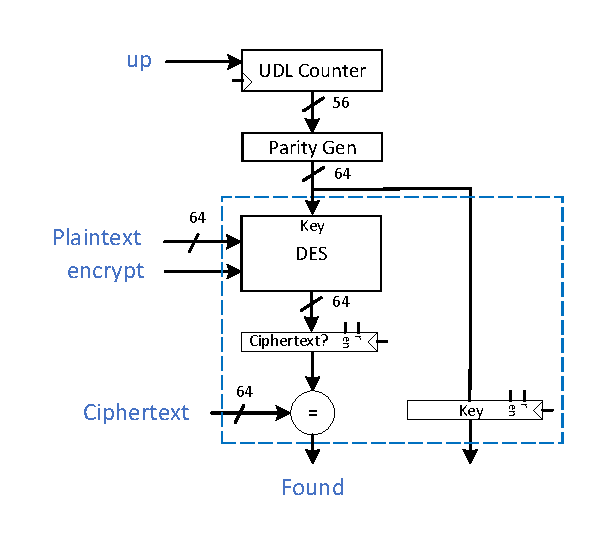
\includegraphics[scale=1.2]{crack_des.pdf}
  \caption{High-level Design of the Top Module (the dotted blue line is the basic
  engine for the cracker)}
  \label{block2.fig}
\end{figure}

The basic idea for the inputs and output includes your move which you
should add through the switches.  As done previously in your labs, you
will need some way of encoding a $3$-bit plaintext and ciphertext into
the switches.  You are welcome to hard code these values into your
design as they will be fixed for each team.  
Since there are only $8$ switches, it would be easier to encode this
as a $3$-bit value for the $8$-bit plaintext/ciphertext.
The suggested signals are listed in the Table in
Table~\ref{io.tbl}, however, they may be modified as needed.
\begin{table}
  \centering
  \begin{tabular}{|c|c|c|c|} \hline
    Signal & Designation & Size [bits] & Description \\ \hline
    \verb!plaintext!  & Input  & $64$  & plaintext \\ \hline
    \verb!ciphertext! & Input  & $64$  & ciphertext \\ \hline
    \verb!Start!      & Input  & $1$  & Start ``cracking'' \\ \hline
    \verb!Found!      & Output & $1$  & Found key signal \\ \hline
    \verb!Key!        & Output & $64$ & Missing key \\ \hline
    \verb!working!    & Output & $1$  & Signal indicating its working \\ \hline
  \end{tabular}
  \caption{Input/Output Signals}
  \label{io.tbl}
\end{table}

The key signal is the \verb!Start! signal that will initiate the
cracking to begin.  So,
the process would be the following for the ``cracker'':
\begin{enumerate}
\item A user would key a $64$-bit input to plaintext and ciphertext
  based on your group (Consult the attached document that lists the
  inputs for each group).  You should probably hard code this value
  into your SystemVerilog Hardware Descriptive Language.
\item The \verb!start! signal would be pushed or enabled to start
  trying to find the missing key.
\item After a set amount of time, the system would respond with the
  correct key given the plaintext and ciphertext.
\end{enumerate}
Again, the \verb!des.sv! module should be intact and not have to
be changed.   You will have to add a couple of registers that will
be provided but the \verb!Enable! signal
has to be designed within the control
signals from the control logic similar to what was discussed in
class.

\subsection{Storing Data}

As mentioned in class, storing data into registers is handled by the
control logic.  Without the control logic, it is very hard for the
datapath element to work properly.  So, you will be tasked to make
sure that the registers get enabled properly.

An enable flip flop or register is just a register that stores data
\textbf{only} if the \verb!EN! signal is asserted.  That is if
\verb!EN=0! any input is not stored into the register and whatever was
inside the register continues to be stored as long as the power is
on.  In order to get this to work correctly, you should make sure you
use good techniques for asserting this \verb!EN! signals from the
control logic.

To store data into the registers \verb!Key! and \verb!Ciphertext?!
registers,
you should store the data if the user has hit the \verb!Start! signal.
But, as explained in class, this should only be done at the right time
and not allow multiple stored data.  The best way to do this is rely
on the \verb!EN! signal and store the value based on your FSM.  The
\verb!working! and \verb!Found! signals
can be used to help you with this to monitor the cracking.  The
process should continue until the datapath compares the computed
ciphertext with the given ciphertext and they are equal.  Then, it
should store the correct key into the \verb!Key! register.  In other
words, a comparator is utilized to indicate to the FSM that it should
stop and store the final result.  There are many ways to build a
comparator in SystemVerilog utilizing what we learned in this class,
however, Chapter 5 in our
textbook~\cite{10.5555/2815529} discusses some other mechansims that
work well.  

For your Finite State Machine (FSM), you should use the \verb!Found!
signal from the comparator
and the \verb!Start! key initiated by the user
to help control the FSM.  There are many
solutions to obtaining the correct FSM design, as the best design is
one that obviously works.  It is also important that, as discussed in
class, you
use some intelligence into your FSM by allowing your FSM to be clocked
on the opposite edge of the clock.  In addition, you should build
intelligence into your FSM so it does not continually try to ``crack''
the key based on a given plaintext and ciphertext.

\subsection{Counters}

Counters are important in that they are sequential logic that provides
a good mechanism to count values.  In fact, some embedded devices uses
counters, called watchdog timers, to help make sure users interact
with devices within a given amount of time.  For this project,  you
will use an up/down/load counter that I will give you.

This counter
will be utilized for generating the key and augmenting the key to the
next value if it is not the correct value.  Although there are many
ways to design counters, I have given you a design that works along
with a sample testbench so you can see how it works.
This counter is also parameterized so you can change the value you
count as well as possibly load a value (perhaps, for use with the
extra credit).

The Up/Down/Load (UDL) counter, shown in Figure~\ref{count.fig} counts
up or down provided the \verb!up! or \verb!down! signal is asserted, respectively.
This is provided that a valid clock is given to its input \verb!clk!.
The SystemVerilog in Figure~\ref{count.fig} also has a neat feature
that allows a pre-determined value to be loaded into the counter via
the \verb!in! signal when \verb!load! is asserted.

The counter along with the flip flops are all given to you.  They are
also parameterized based on the \verb!WIDTH! defined value, as
discussed in class.  It would be advisable to use the \verb!flopenr!
flip flop as it has an enable and reset pin that you should utilize
along with the FSM.

The counter outputs a $56$ bit count that is utilized for the key,
since DES requires odd parity~\cite{fips463}, we need to create parity to generate
the values correctly to the DES engine.  You should create another
module that calculates the parity and produces the correct parity for
the count.  This can be done easily with SystemVerilog utilizing
simple RTL-level constructs.
\begin{figure}
  \centering
  {\footnotesize
\begin{verbatim}
  module UDL_Count  #(parameter WIDTH=8) 
   (clk, rst, up, down, load, in, out) ;

   input logic              clk;
   input logic              rst;
   input logic              up;
   input logic              down;
   input logic              load;
   input logic [WIDTH-1:0]  in;
   
   output logic [WIDTH-1:0] out;

   logic [WIDTH-1:0]        next;
   
   flop #(WIDTH) count(clk, next, out);

   always_comb begin
      if (rst)
        next = {WIDTH{1'b0}};
      else if (load)
        next = in;
      else if (up)
        next = out + 1'b1;
      else if (down)
        next = out - 1'b1;
      else
        next = out;
   end // always@ *
   
endmodule 
\end{verbatim}
}
\caption{Up/Down/Load (UDL) counter in SystemVerilog}
\label{count.fig}
\end{figure}


\section{Tasks}

Most of the modules have been given to you to help you understand the
problem better.   In fact, we have given much of the project for you
in this text.  You just have to implement and test it with a
testbench.  The tasks of the project are as follows:
\begin{enumerate}
  \item To make things work effectively and not cause any issues, it
    may be prudent to have the    
    plaintext and ciphertext registered.  You
    can, of course, hard code these values in to make it easier, if needed.
\item  Integrate Figure~\ref{block2.fig} with the \verb!des.sv!
  module.  Although you could design the next step, it is easier to
  test your design without the control logic first.  I would recommend
  using this approach by adding the control signals verbatim in the
  testbench before integrated the FSM in the next step.
\item Design a control logic presumably with a FSM to have it work
  correctly.
  \item Integrate both the datapath from Step~$1$ and the control
    logic from Step~$2$ using the clocking methodology discussed in
    class.
    You can call this design \verb!top.sv!.  This should have both your datapath
    and control logic in it.
  \item Test  your design completely with a testbench.  
  \item Once your design completely works, implement the design on
    the DSDB board.  You should probably use the switches, push
    buttons, LEDs and also use the
    seven segment display to output \verb!plaintext!, \verb!ciphertext!
    and \verb!Key!.  Remember, to use the LEDs to help you
    debug your design.      
\end{enumerate}

Again, the process here is not difficult.  If you need to work out any
of the procedures or ask me to inspect your design, I would recommend
stopping by to ask questions or advice.  I would not advise waiting
until the last week to start as I might be busy with
end-of-the-semester duties and starting early is the best practice.

Each team will be given a different key based on a plaintext and
ciphertext.  This is documented in an additional document that lists
the message and its associated ciphertext by Team.  Please consult
this document to make sure you are using the right values as it will
impact your final score.

\subsection{Extra Credit}

There are lots of opportunities for extra credit with this project.
But, please, first focus on completing the baseline project before
attempting the extra credit option.  One of the advantages of digital
logic is that many bits can be computed in parallel and then chosen
later to be correct or incorrect.  The blue blox in
Figure~\ref{block2.fig} can be replicated as many times as needed to
compute the design faster.

Because Field Programmable Gate Arrays
(FPGAs) can contain many millions of logic gates, you could
theoretically replicate this blue block several times to compute the key much
faster.  However, you will have to think about how to distribute the
random key generation to test it quicker and more efficiently.  A
recommendation is to use the logarithmic approach we saw in class
with the shifter to help create a more efficient method for
implementing this approach.

However, replicating the design in Figure~\ref{block2.fig} also
necessitates careful redesign of the FSM/control logic to make sure
the correct key is produced.  For those that want to try this option,
I will give a prize for the design that produces the key in the
smallest number of steps.

\section{Demo and Lab Report}

Please work
consistently throughout the final weeks of the semester to make sure
you complete the project on time.
I will also give extra credit to those that put a little effort into
making an outstanding design and showcasing their project in detail.
You could also potentially discuss other symmetric and asymmetric
key algorithms and how DES laid the groundwork for other more
current cryptographic algorithms, such as the Advanced Encryption
Standard~\cite{10.5555/1721909}.

You are also required to submit a final report of your design using
the lab rubric.  You should remember to submit your lab report
to Canvas for
your team, but please also submit your team evaluation, as well.
Beware; no
late projects will be accepted and if you miss submitting your project
on time, you will receive a $0$ for your project grade!  This
procedure should be similar to what you are using for your labs.
You should also take a printout of your waveform 
from your ModelSim simulation.  
Only one of your team members should upload
the files, lab report, and team assessment.  Also, please make sure you
hand in all files, including your HDL, testbenches, and other
important files you wish for us to see.  You should also identify in
your lab report the
correct key that you found through your cracker.  

Although a demo is not required, if you set up a demo with me, I will
give you extra credit for it.  You could also create a video on your
cell phone documenting your project.  Any additional item you want to
create for your project will be counted towards extra credit and its a
way to increase your score, if needed, for a missed homework or other
points you got deducted earlier in the semester.  It is also good to
document these items, as discussed in class, for future internships
and jobs; therefore, work  hard to work hard on this project!

Please contact
the James Stine
(james.stine@okstate.edu) 
for more help.  Your
code should be
readable and well-documented. In addition, please turn in additional
test cases or any other added item that you used. 
Please also remember to document everything in your Lab Report using
the information found in the Grading Rubric.

   
\bibliographystyle{IEEEbib}
\bibliography{project}

\end{document}
